\documentclass{beamer}
\usepackage[utf8]{inputenc}

\usetheme{Madrid}
\usecolortheme{default}
\usepackage{amsmath,amssymb,amsfonts,amsthm}
\usepackage{mathtools}
\usepackage{txfonts}
\usepackage{tkz-euclide}
\usepackage{listings}
\usepackage{adjustbox}
\usepackage{array}
\usepackage{tabularx}
\usepackage{gvv}
\usepackage{lmodern}
\usepackage{circuitikz}
\usepackage{tikz}
\usepackage{graphicx}

\setbeamertemplate{page number in head/foot}[totalframenumber]

\usepackage{tcolorbox}
\tcbuselibrary{minted,breakable,xparse,skins}



\definecolor{bg}{gray}{0.95}
\DeclareTCBListing{mintedbox}{O{}m!O{}}{%
  breakable=true,
  listing engine=minted,
  listing only,
  minted language=#2,
  minted style=default,
  minted options={%
    linenos,
    gobble=0,
    breaklines=true,
    breakafter=,,
    fontsize=\small,
    numbersep=8pt,
    #1},
  boxsep=0pt,
  left skip=0pt,
  right skip=0pt,
  left=25pt,
  right=0pt,
  top=3pt,
  bottom=3pt,
  arc=5pt,
  leftrule=0pt,
  rightrule=0pt,
  bottomrule=2pt,
  toprule=2pt,
  colback=bg,
  colframe=orange!70,
  enhanced,
  overlay={%
    \begin{tcbclipinterior}
    \fill[orange!20!white] (frame.south west) rectangle ([xshift=20pt]frame.north west);
    \end{tcbclipinterior}},
  #3,
}
\lstset{
    language=C,
    basicstyle=\ttfamily\small,
    keywordstyle=\color{blue},
    stringstyle=\color{orange},
    commentstyle=\color{green!60!black},
    numbers=left,
    numberstyle=\tiny\color{gray},
    breaklines=true,
    showstringspaces=false,
}
%------------------------------------------------------------
%This block of code defines the information to appear in the
%Title page
\title %optional
{2.10.12}

%\subtitle{A short story}

\author % (optional)
{Pratik R-AI25BTECH11023}



\begin{document}


\frame{\titlepage}
\begin{frame}{Question}
A unit vector perpendicular to the plane determined by the points
$P\brak{1,-1,2}$,$Q\brak{2,0,-1}$ and $R\brak{0,2,1}$ is 
\end{frame}




\begin{frame}{Solution}
\textbf{solution}:\\

According to the question, 
Given the position vectors,
\begin{align}
    \vec{P}=\myvec{1\\-1\\2};
    \vec{Q}=\myvec{2\\0\\-1};
    \vec{R}=\myvec{0\\2\\1}
\end{align}
Let the perpendicular vector be $\vec{n}^T=\myvec{n_1&&n_2&&n_3}$
\begin{align}
    \because \vec{n}^\top \vec{P}=1 \\
    \vec{n}^\top \vec{Q}=1 \\
    \vec{n}^\top \vec{R}=1 
\end{align}
\end{frame}
\begin{frame}{Solution}
\begin{align}
    \therefore \myvec{\vec{P}^\top \\\vec{Q}^\top \\\vec{R}^\top}\vec{n}= \myvec{1 \\ 1}
\end{align}
\begin{align}
    \therefore \myvec{\vec{P} & \vec{Q} & \vec{R}}^\top \vec{n}= \myvec{1 \\ 1}
\end{align}
\begin{align}
    \myvec{1&&-1&&2\\2&&0&&-1 \\ 0&&2&&1} \vec{n}= \myvec{1 \\ 1 \\ 1}
\end{align}
\end{frame}
\begin{frame}{Solution}
The augmented matrix for the above system of Equations is given by
\begin{align}
    \myvec{1&-1&2&&1\\2&0&-1&&1\\0&2&1&&1} 
\end{align}

Solving equation 0.8 we get
\begin{align}
    \vec{n}=\frac{1}{3}\myvec{2\\1\\1}
\end{align}
\end{frame}
\begin{frame}{Solution}
The unit vector perpendicular to the plane is given by $\vec{x}$
\begin{align}
     \vec{x}= \frac{\vec{n}}{||n||} =   \frac{1}{\sqrt{6}}\myvec{2\\1\\1}
\end{align}
\end{frame}

\begin{frame}{Plot}
    \begin{figure}[H]
    \centering
    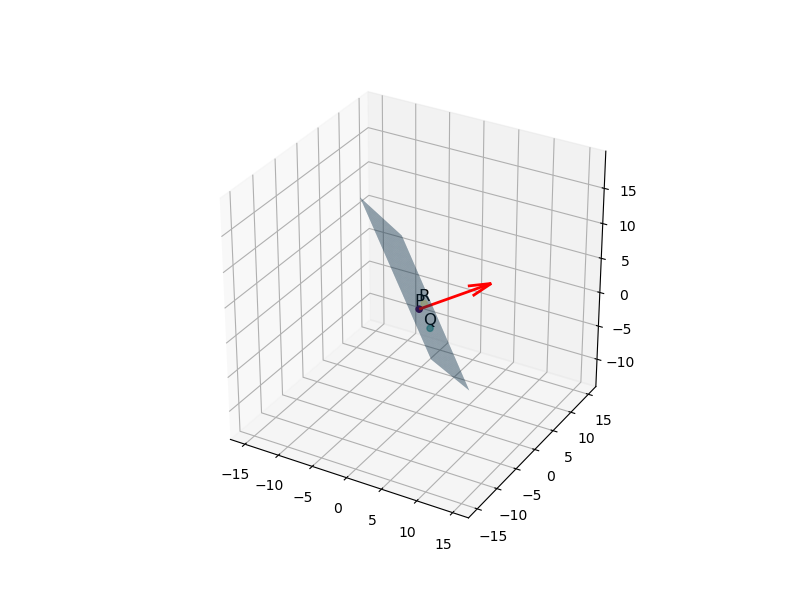
\includegraphics[width=0.6\columnwidth]{../figs/fig.png}
    \label{fig:1}
\end{figure}
\end{frame}

\begin{frame}[fragile]
    \frametitle{C Code - unit normal vector for plane}

    \begin{lstlisting}
#include <stdio.h>
#include <math.h>

int main() {
    // Coordinates of the points
    double P[3] = {1, -1, 2};
    double Q[3] = {2, 0, -1};
    double R[3] = {0, 2, 1};
    \end{lstlisting}
\end{frame}
\begin{frame}[fragile]

    \frametitle{C Code - unit normal vector for plane}
    \begin{lstlisting}
        / Store points to a file (no labels, just coordinates)
    FILE *fptr;
    fptr = fopen("output.data", "w");
    if (fptr == NULL) {
        printf("Error opening file!\n");
        return 1;
    }
    fprintf(fptr, "%lf %lf %lf\n", P[0], P[1], P[2]);
    fprintf(fptr, "%lf %lf %lf\n", Q[0], Q[1], Q[2]);
    fprintf(fptr, "%lf %lf %lf\n", R[0], R[1], R[2]);
    fclose(fptr);
    \end{lstlisting}
\end{frame}
\begin{frame}[fragile]
    \frametitle{C Code - unit normal vector for plane}

    \begin{lstlisting}
/
    // Compute vectors PQ and PR
    double PQ[3], PR[3];
    for (int i = 0; i < 3; i++) {
        PQ[i] = Q[i] - P[i];
        PR[i] = R[i] - P[i];
    }

    // Cross product PQ x PR
    double N[3];
    N[0] = PQ[1]*PR[2] - PQ[2]*PR[1];
    N[1] = PQ[2]*PR[0] - PQ[0]*PR[2];
    N[2] = PQ[0]*PR[1] - PQ[1]*PR[0];

    \end{lstlisting}
\end{frame}
    \begin{frame}[fragile]
    \frametitle{C Code - unit normal vector for plane}

    \begin{lstlisting}

    // Magnitude of the vector N
    double mag = sqrt(N[0]*N[0] + N[1]*N[1] + N[2]*N[2]);

    // Unit vector
    double unit[3];
    for (int i = 0; i < 3; i++) {
        unit[i] = N[i] / mag;
    }

    printf("Unit vector perpendicular to the plane: (%lf, %lf, %lf)\n", unit[0], unit[1], unit[2]);
    return 0;
}
    \end{lstlisting}
\end{frame}
    






\begin{frame}[fragile]
    \frametitle{Python Code}
    \begin{lstlisting}
import sys                                          #for path to external scripts

import numpy as np
import numpy.linalg as LA
import matplotlib.pyplot as plt
import matplotlib.image as mpimg
from mpl_toolkits.mplot3d import Axes3D

#local imports
from line.funcs import *
#from triangle.funcs import *
#from conics.funcs import circ_gen

#if using termux
import subprocess
import shlex
#end if
    \end{lstlisting}
\end{frame}

\begin{frame}[fragile]
    \frametitle{Python Code}
    \begin{lstlisting}
# Read points from output.data file
points = []
with open('output.data', 'r') as file:
    for line in file:
        coords = list(map(float, line.split()))
        points.append(coords)

# Convert to numpy arrays with required shape
P = np.array(points[0]).reshape(-1, 1)
Q = np.array(points[1]).reshape(-1, 1)
R = np.array(points[2]).reshape(-1, 1)

    \end{lstlisting}
\end{frame}

\begin{frame}[fragile]
    \frametitle{Python Code}
    \begin{lstlisting}
# Create a figure and a 3D Axes
fig = plt.figure(figsize=(8, 6))
ax = fig.add_subplot(111, projection='3d')

a, b, c, d = 2, 1, 1, -3  # coefficients of the plane equation: ax + by + cz + d = 0

# Generate grid points for x and y
x = np.linspace(-5, 5, 50)
y = np.linspace(-5, 5, 50)
X, Y = np.meshgrid(x, y)

# Calculate corresponding z values for each (x, y) pair to satisfy the plane equation
Z = (-a*X - b*Y - d) / c

    \end{lstlisting}
\end{frame}

\begin{frame}[fragile]
    \frametitle{Python Code}
    \begin{lstlisting}
# Plot the plane
ax.plot_surface(X, Y, Z, alpha=0.5)

#Generating all lines
#x_BC = line_gen(Q,R)

#Plotting all lines
#ax.plot(x_QR[0,:],x_QR[1,:], x_QR[2,:],label='$BC$')

# Scatter plot
colors = np.arange(2, 5)  # Example colors
tri_coords = np.block([P,Q,R])  # Stack P,Q,R vertically
ax.scatter(tri_coords[0, :], tri_coords[1, :], tri_coords[2, :], c=colors)
vert_labels = ['P', 'Q', 'R']
ax.quiver(1,-1,2, 2,1,1, color='r', linewidth=2, label='n')
    \end{lstlisting}
\end{frame}

\begin{frame}[fragile]
    \frametitle{Python Code}
    \begin{lstlisting}
for i, txt in enumerate(vert_labels):
    # Annotate each point with its label and coordinates
    ax.text(tri_coords[0, i], tri_coords[1, i], tri_coords[2, i],f'{txt}',fontsize=12, ha='center', va='bottom')
    #ax.text(tri_coords[0, i], tri_coords[1, i], tri_coords[2, i], f'{txt}\n({tri_coords[0, i]:.0f}, {tri_coords[1, i]:.0f}, {tri_coords[2, i]:.0f})',
    #         fontsize=12, ha='center', va='bottom')


ax.spines['top'].set_color('none')
ax.spines['left'].set_position('zero')
ax.spines['right'].set_color('none')
ax.spines['bottom'].set_position('zero')

    \end{lstlisting}
\end{frame}
\begin{frame}[fragile]
    \frametitle{Python Code}
    \begin{lstlisting}

ax.set_xlim(-4, 4)  # Adjust limits based on your data
ax.set_ylim(-4, 4)  # Adjust limits based on your data
ax.set_zlim(-4, 4)  # Adjust limits based on your data
ax.set_box_aspect([1,1,1])  
'''
ax.spines['left'].set_visible(False)
ax.spines['right'].set_visible(False)
ax.spines['top'].set_visible(False)
ax.spines['bottom'].set_visible(False)
plt.xlabel('$x$')
plt.ylabel('$y$')
plt.legend(loc='best')
'''
plt.grid() # minor
plt.axis('equal')

plt.savefig('../figs/fig.png')
    \end{lstlisting}
\end{frame}




\end{document}